% Created 2020-11-05 Thu 11:50
% Intended LaTeX compiler: pdflatex
\documentclass[unicode, 12pt, xdvipdfmx, aspectratio=43]{beamer}
\usepackage[utf8]{inputenc}
\usepackage[T1]{fontenc}
\usepackage{graphicx}
\usepackage{grffile}
\usepackage{longtable}
\usepackage{wrapfig}
\usepackage{rotating}
\usepackage[normalem]{ulem}
\usepackage{amsmath}
\usepackage{textcomp}
\usepackage{amssymb}
\usepackage{capt-of}
\usepackage{hyperref}
\usepackage[backend=bibtex, style=authoryear, maxcitenames=2]{biblatex}
\addbibresource{../resources/anthology.bib}
\addbibresource{../resources/my.bib}
\let\oldcite\cite
\renewcommand{\cite}[1]{{\scriptsize\reffont{(\oldcite{#1})}}}
\newcommand{\citet}[2][\footnotesize]{{\reffont#1\citeauthor*{#2} (\citeyear{#2})}}
\newcommand{\mycite}[1]{{\scriptsize\reffont({\citeauthor*{#1}, \citeyear{#1}})}}
\newcommand{\myfootcite}[1]{\footnote{\tiny\reffont\citetitle{#1}, \citeauthor*{#1}, \citeyear{#1}.}}
\usepackage{hyperref}
\usetheme{metropolis}
\setbeamertemplate{items}[default]
\setbeamertemplate{itemize item}{\small\raise0.5pt\hbox{$\blacksquare$}}
\setbeamertemplate{itemize subitem}{\footnotesize\raise1.5pt\hbox{$\bullet$}}
\setbeamertemplate{itemize subsubitem}{\scriptsize\raise1.5pt\hbox{$\blacktriangleright$}}
\setbeamertemplate{enumerate item}{\textbf{(\arabic{enumi})}}
\addtolength{\skip\footins}{6pc plus 10pt}
\usepackage{xltxtra}
\usepackage{booktabs}
\usepackage[absolute,overlay]{textpos}
\usepackage{pgfpages}
\usepackage{tikz}
\usepackage{tikz-dependency}
\usetikzlibrary{arrows.meta, matrix, positioning, fit, calc, backgrounds, shapes.callouts}
\usepackage{pgfgantt}
\usepackage{adjustbox}
\usepackage{array}
\usepackage[linguistics]{forest}
\newcommand{\highlightcap}[3][blue]{\tikz[baseline=(x.base)]{\node[rectangle,rounded corners,fill=#1!20](x){#2} node[below=0.5ex of x, color=#1]{#3};}}
\newcommand{\highlight}[2][blue]{\tikz[baseline=(x.base)]{\node[rectangle,rounded corners,fill=#1!20](x){#2};}}
\newcommand{\calloutbase}[2]{\tikz[remember picture, baseline=(#1.base)]{\node(#1) {#2};}}
\newcommand{\calloutpos}[2]{\tikz[remember picture, overlay]{\node[below=0cm of #1] {#2};}}
\newcommand{\calloutbelow}[3][blue]{\tikz[remember picture, overlay]{\node[rectangle callout, rounded corners, fill=#1!10, callout absolute pointer={(#2.south)}, below=of #2] {#3};}}
\usepackage{xcolor}
\definecolor{myalert}{HTML}{AD003D}
\definecolor{mDarkTeal}{HTML}{23373b}
\definecolor{mLightGreen}{HTML}{14B03D}
\usefonttheme{professionalfonts}
\usepackage[T1]{fontenc}
\usepackage{fontspec}
\XeTeXlinebreaklocale "ja"
\usepackage{xeCJK}
\setsansfont[BoldFont={Fira Sans Bold}]{Fira Sans Book}
\setCJKmainfont{Noto Sans CJK JP}
\setCJKsansfont{Noto Sans CJK JP}
\setCJKromanfont{Noto Serif CJK JP}
\xeCJKDeclareCharClass{CJK}{`※}
\newfontfamily\firasans{Fira Sans}
\newfontfamily\emojifont{Noto Emoji}
\newfontfamily\octicons{github-octicons}
\newfontfamily\materials{Material Icons}
\newfontfamily\faicons{FontAwesome}
\newfontfamily\reffont{Times New Roman}
\usepackage{amssymb}
\usepackage{mathfont}
\usepackage{bbm}
\renewcommand{\baselinestretch}{1.3}
\usetheme{default}
\author{出口 ~ 祥之 \\ \lower2.0pt\hbox{\materials} \texttt{deguchi@ai.cs.ehime-u.ac.jp}}
\date{2020/11/05 ~ 二宮研 論文輪読会}
\title{Nearest Neighbor Machine Translation}
\subtitle{(Khandelwal et al., 2020)}
\institute{}
\hypersetup{
 pdfauthor={出口 ~ 祥之 \\ \lower2.0pt\hbox{\materials} \texttt{deguchi@ai.cs.ehime-u.ac.jp}},
 pdftitle={Nearest Neighbor Machine Translation},
 pdfkeywords={},
 pdfsubject={},
 pdfcreator={Emacs 27.1 (Org mode 9.3.7)}, 
 pdflang={English}}
\begin{document}

\maketitle

\begin{frame}[label={sec:org2fb6839}]{\hbox{\octicons} Links}
\begin{block}{\raise0.5pt\hbox{\octicons} Paper}
\begin{block}{\url{https://arxiv.org/abs/2010.00710}}
\end{block}
\end{block}
\end{frame}
\begin{frame}[label={sec:org8fc6652}]{Introduction}
\vspace{-0.2cm}
\begin{block}{k近傍法を利用した生成により翻訳性能の大幅改善}
\vspace{-0.2cm}
\small
\begin{itemize}
\item 翻訳時に訓練データを参照してk近傍法を適用 \vspace{-0.2cm}
\begin{itemize}
\item 翻訳時の処理のみが変わるため,追加の訓練無しで従来の訓練済み NMT モデルをそのまま利用可能
\end{itemize}
\item 翻訳性能の大幅改善
\begin{itemize}
\item SOTAな独英翻訳システムと比較して +1.5 BLEU \%
\item 多言語翻訳システムにおいて英独・中英・英中翻訳などで +3 BLEU \%
\item ドメインに特化したデータ (翻訳のドメイン適応) に対して平均で +9.2 BLEU \%
\end{itemize}
\end{itemize}
\end{block}
\end{frame}
\begin{frame}[label={sec:orgcacf851}]{k-Nearest Neighbor (kNN)}
\begin{block}{最も近い例に基づいた分類法}
\vspace{0.5cm}
距離が近いサンプル \(k\) 個を参照し,最も一般的なクラスを割り当てる

\begin{columns}
\begin{column}{0.65\columnwidth}
\begin{block}{例: 赤三角と青四角の 2 クラス分類}
\begin{description}
\item[{\(k = 3\) のとき}] 緑丸→赤三角クラス
\item[{\(k = 5\) のとき}] 緑丸→青四角クラス
\end{description}
\end{block}
\end{column}

\begin{column}{0.35\columnwidth}
\begin{center}
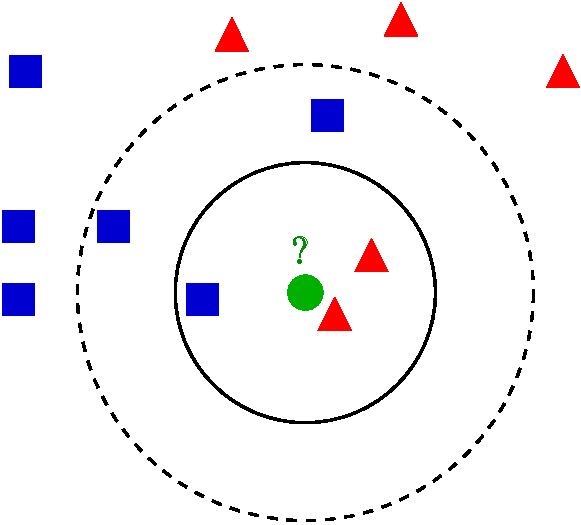
\includegraphics[width=\linewidth]{./figure/KnnClassification.pdf}
\end{center}
\tiny
\url{https://en.wikipedia.org/wiki/K-nearest\_neighbors\_algorithm} (CC-BY-SA 3.0; by Antti Ajanki)
\end{column}
\end{columns}
\end{block}
\end{frame}

\section{Proposed Method}
\label{sec:orge527d37}
\begin{frame}[label={sec:org927cd44}]{Nearest Neighbor Machine Translation}
\begin{block}{翻訳時,ステップ毎に k 近傍法を適用して探索}
\begin{center}
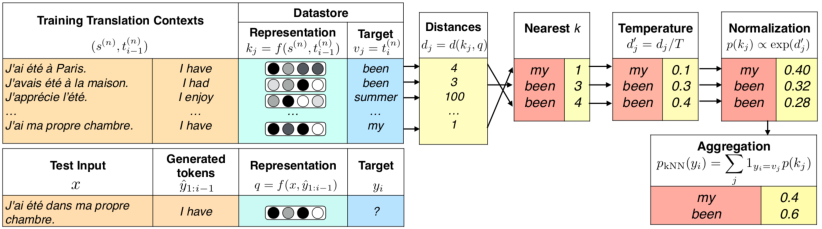
\includegraphics[width=\linewidth]{./figure/Figure1.pdf}
\end{center}

\begin{description}
\item[{データストア:}] 訓練データ (対訳コーパス) の目的言語文の各単語位置における中間表現を事前に作成
\item[{\(q = f(x, \hat{y}_{1:i-1})\) :}] 翻訳時の各ステップにおける中間表現
\end{description}
\end{block}
\end{frame}

\begin{frame}[label={sec:orge2d1e55}]{Nearest Neighbor Machine Translation}
\begin{center}
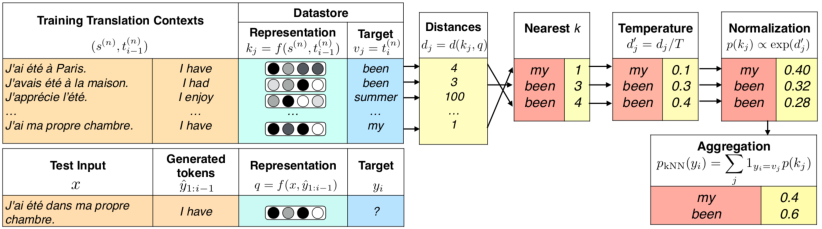
\includegraphics[width=\linewidth]{./figure/Figure1.pdf}
\end{center}
\metroset{block=fill}
\renewcommand{\baselinestretch}{1.0}
\small
\begin{block}{翻訳時の動作}
\begin{enumerate}
\item \(q\) とデータストア内の中間表現との距離から \(k\) 近傍を獲得
\item \(k\) 近傍内の各距離に対して温度付き softmax 関数を適用
\item 2. の計算結果を集約し,確率に変換
\item モデルの出力確率と 3. の確率を線形補間
\end{enumerate}

\renewcommand{\baselinestretch}{1.3}
\end{block}
\end{frame}

\begin{frame}[label={sec:orgca87ccc}]{Datastore creation}
\begin{block}{全翻訳過程の中間表現を事前に作成}
\begin{equation*}
  (\highlight[orange]{$\mathcal{K}$},\highlight[mLightGreen]{$\mathcal{V}$}) = \{ (\highlight[orange]{$f(s, t_{1:i-1})$}, \highlight[mLightGreen]{$t_i$}), \forall t_i \in t \mid (s, t) \in (\mathcal{S}, \mathcal{T}) \} 
\end{equation*}
※ \(f\) : NMT モデル (デコーダの中間表現を返す) \\
※ \((\mathcal{S}, \mathcal{T})\) : 対訳コーパス

\small
\begin{itemize}
\item \highlight[orange]{キー: 中間表現},\highlight[mLightGreen]{値: キーから生成される正解トークン $t_i$}
\item 原言語文の情報はキーの中に暗黙的に含まれる
\end{itemize}
\end{block}
\end{frame}

\begin{frame}[label={sec:org2796485}]{Generation}
\small
\begin{block}{温度付き softmax により距離に基づいた確率を算出}
\begin{equation*}
  \highlight[cyan]{$p_{kNN}(y_i | x, \hat{y}_{1:i-1})$} \propto \sum_{(k_j, v_j) \in \mathcal{N}} \mathbbm{1}_{y_i = v_j} \exp \left( \frac{ \highlight[orange]{$-d(k_j, f(x, \hat{y}_{1:i-1}))$} }{T} \right)
\end{equation*}
※ \(\hat{y}\) : 翻訳時の生成済みトークン \\
※ \(\mathcal{N}\) : 距離関数に \alert{最小自乗誤差} を用いて得る \(k\) 近傍中間表現

\vspace{1cm}
\end{block}
\begin{block}{NMT モデルの出力確率 \highlight[mLightGreen]{ $p_{MT}(y_i | x, \hat{y}_{1:i-1})$ } と線形補間}
\begin{equation*}
  p(y_i | x, \hat{y}_{1:i-1}) = \lambda \highlightcap[cyan]{$p_{kNN}(y_i | x, \hat{y}_{1:i-1})$}{距離に基づく確率} + (1 - \lambda) \highlightcap[mLightGreen]{$p_{MT}(y_i | x, \hat{y}_{1:i-1})$}{モデル出力確率}
\end{equation*}
\end{block}
\end{frame}

\begin{frame}[label={sec:orgc7e6d6c}]{Experimental Setup}
\begin{block}{データセット}
\begin{enumerate}
\item 通常の翻訳 (WMT'19 De-En)
\item 多言語翻訳 (訓練: CCMatrix,評価: newstest2018, newstest2019, TED Talks)
\item ドメイン適応 (multi-domains; Medical, Law, IT, Koran, Subtitles)
\end{enumerate}
\end{block}

\begin{block}{モデル}
\begin{description}
\item[{NMT システム}] Transformer (\texttt{Fairseq})
\end{description}
\end{block}
\end{frame}

\begin{frame}[label={sec:org0e475b1}]{kNN-MT, Computational Cost}
\small
\begin{description}
\item[{\(k\) NN-MT}] \texttt{Faiss} (高速な k 近傍探索ライブラリ) を使用
\begin{itemize}
\item キー: Transformer 最終層 FFN への入力
\begin{itemize}
\item 多言語翻訳: キー 5M,131K クラスタ
\item ドメイン適応: キー 1M,4K クラスタ
\end{itemize}
\item 64 近傍,32 クラスタを探索 ( \(k = 64\) )
\end{itemize}
\end{description}

\begin{block}{計算時間と引き換えに追加訓練無しで翻訳性能を改善}
\begin{description}
\item[{データストア作成}] 事前に全てのサンプルに対して一度順方向に計算すればよい \\ (訓練 1 エポック分と同等のコスト)
\item[{翻訳時}] データストア全体 (10 億のオーダー) から 64 近傍を得るため,生成速度が 2 桁程遅くなる
\end{description}
\end{block}
\end{frame}

\begin{frame}[label={sec:orgc8277be}]{Experiments}
\begin{block}{WMT'19 De-En}
\begin{center}
\begin{tabular}{ll}
\toprule
モデル & BLEU (\%)\\
\midrule
baseline & 37.59\\
+kNN-MT & \textbf{39.08 (+1.5)}\\
\bottomrule
\end{tabular}
\end{center}

\begin{itemize}
\item 追加の訓練無しで 1.5 BLEU \% の性能改善
\end{itemize}
\end{block}
\end{frame}

\begin{frame}[label={sec:org2f786f8}]{Multilingual Machine Translation}
\begin{block}{評価する言語対と同じ言語対のデータストアを構築}
\begin{center}
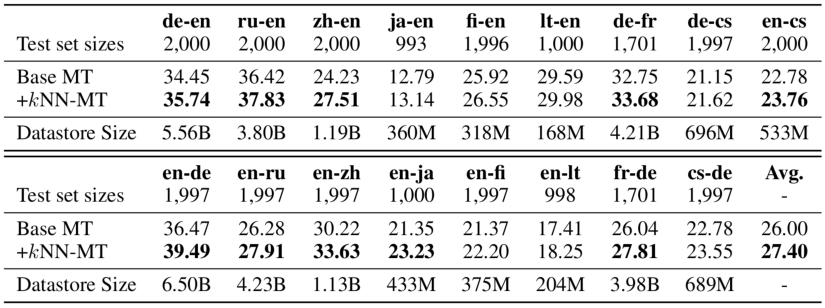
\includegraphics[width=\linewidth]{./figure/Table1.pdf}
\end{center}
\end{block}
\end{frame}

\begin{frame}[label={sec:org4a553ea}]{Multilingual Machine Translation}
\begin{block}{原言語側を英語にしてデータストアを構築}
\begin{center}
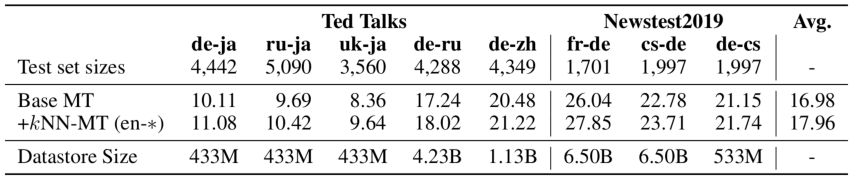
\includegraphics[width=\linewidth]{./figure/Table2.pdf}
\end{center}
\end{block}
\end{frame}

\begin{frame}[label={sec:org7c61fc5}]{Domain Adaptation}
\begin{block}{5 つの異なるドメインに対し zero-shot 翻訳}
\begin{center}
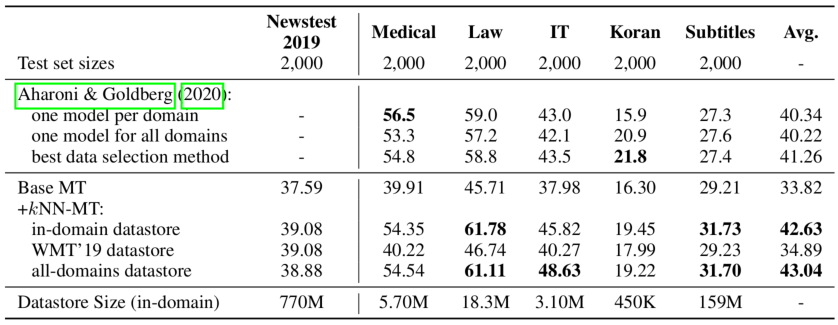
\includegraphics[width=\linewidth]{./figure/Table3.pdf}
\end{center}
\end{block}
\end{frame}

\begin{frame}[label={sec:org87e85e3}]{Tuning kNN-MT (on validation set)}
\small
\begin{block}{探索幅 \(k\)}
\begin{itemize}
\item 実験では 64 で固定
\item 大きくしても性能は変わらず,下がることも (ノイズ?)
\end{itemize}
\end{block}

\begin{block}{Softmax の温度パラメータ \(T\)}
\begin{columns}
\begin{column}{0.6\columnwidth}
\begin{itemize}
\item \(T\) \textbf{が大きくなるほど:}
\begin{itemize}
\item 分布が平坦になる
\item コンテクストへの過剰適合が抑えられる
\item 多様性が高まる
\end{itemize}
\end{itemize}
\end{column}
\begin{column}{0.4\columnwidth}
\begin{center}
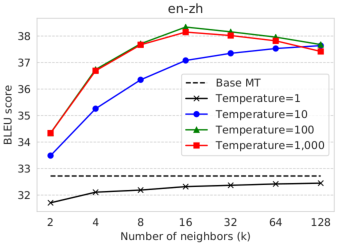
\includegraphics[width=\linewidth]{./figure/Figure2.pdf}
\end{center}
\end{column}
\end{columns}
\end{block}
\end{frame}

\begin{frame}[label={sec:org630e755}]{Tuning kNN-MT (on validation set)}
\begin{block}{データストアの大きさと翻訳性能}
\begin{center}
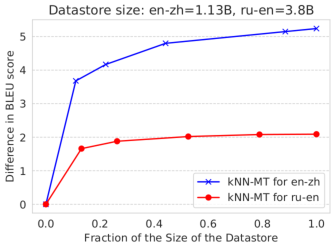
\includegraphics[width=0.5\linewidth]{./figure/Figure3.pdf}
\end{center}
\end{block}
\end{frame}

\begin{frame}[label={sec:org2b8f158}]{Qualitative Analysis}
\begin{block}{kNN 分布のみで生成される場合 ( \(\lambda = 1\) )}
\vspace{-0.5cm}
\begin{center}
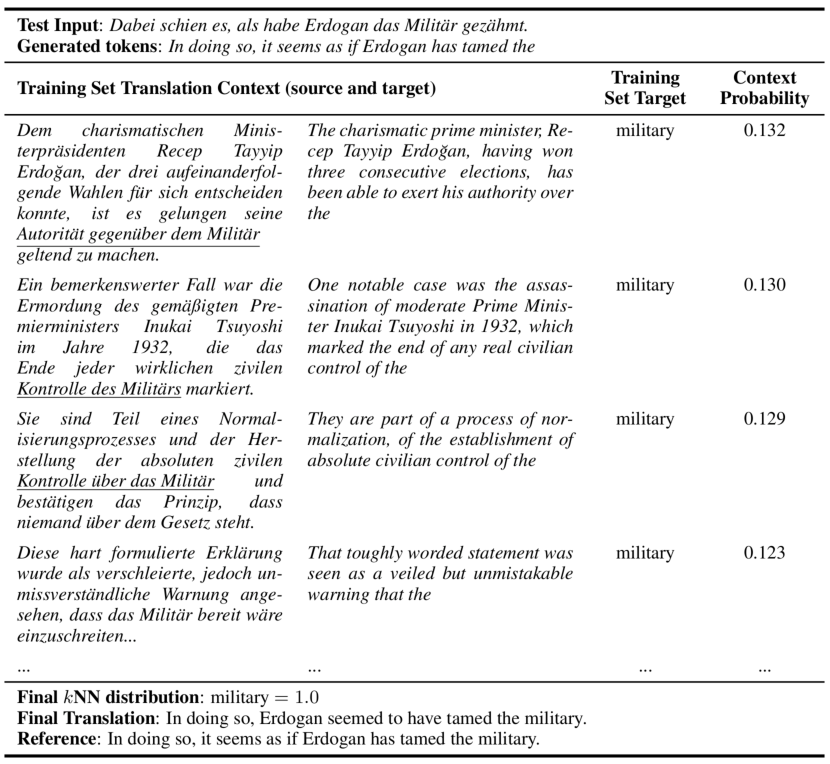
\includegraphics[width=0.75\linewidth]{./figure/Figure4.pdf}
\end{center}
\end{block}
\end{frame}

\begin{frame}[label={sec:org07b7c47}]{Related Work (Retrieval in Translation)}
\renewcommand{\baselinestretch}{1.2}
\begin{block}{NMT による翻訳と検索の組み合わせ}
\begin{itemize}
\item 対訳コーパスから \(n\text{-gram}\) 翻訳句を検索 \myfootcite{zhang-etal-2018-guiding}
\item キャッシュに保存した翻訳履歴から検索 \myfootcite{tu-etal-2018-learning}
\end{itemize}
\end{block}

\begin{block}{用例に基づく機械翻訳}
\begin{itemize}
\item アナロジーに基づく機械翻訳 \myfootcite{nagao-1984-framework}
\item 編集距離に基づく似た原言語文から翻訳例を検索 \myfootcite{gu-etal-2018-search}
\item NMT と翻訳メモリ検索の組み合わせ \myfootcite{bulte-tezcan-2019-neural} \myfootcite{xu-etal-2020-boosting}
\end{itemize}

\vspace{0.3cm}
\renewcommand{\baselinestretch}{1.3}
\end{block}
\end{frame}

\begin{frame}[label={sec:orgdfbc8f5}]{Conclusion}
\begin{block}{追加訓練無しに従来の NMT モデルに適用できる \\ 新たな翻訳法 kNN-MT を提案}
\begin{itemize}
\item 翻訳時,NMT モデルの中間表現と近いコンテクストベクタを k 近傍法により探索
\item kNN-MT による確率とモデルの出力確率との線形補間から出力単語を得ることで翻訳性能を大幅改善
\end{itemize}
\end{block}

\begin{block}{今後の課題}
\begin{itemize}
\item 手法の効率化
\begin{itemize}
\item 頻出する単語をダウンサンプリングするなど
\end{itemize}
\end{itemize}
\end{block}
\end{frame}
\end{document}